\section{Methodology}

\lstset{
  basicstyle=\small\ttfamily,
  captionpos=b,
  frame=single,
  breaklines=true,
  showstringspaces=false,
  aboveskip=2.5pt,
  belowskip=2pt
}

\subsection{Hyperparameters}

\subsection{Data collection and preprocessing}

\subsection{Model architecture}
\[
    input\_dim = \sum_{j=1}^{m} \begin{cases} 1 & \text{if feature}_j \text{ is in the vocabulary} \\ 0 & \text{otherwise} \end{cases}
\]
\indent Sum of ones and zeros, where each 1 indicates the presence of unique feature in the vocabulary.

\begin{lstlisting}[language=Python, caption={Modell Python kód tartalma}, label=modell]
    class TextClassifier(nn.Module):
        def __init__(self, input_dim):
            super(TextClassifier, self).__init__()
            self.fc1 = nn.Linear(input_dim, 64)
            self.fc2 = nn.Linear(64, 32)
            self.fc3 = nn.Linear(32, 2)

        def forward(self, x):
            x = torch.relu(self.fc1(x))
            x = torch.relu(self.fc2(x))
            x = self.fc3(x)
            return x
\end{lstlisting}
\begin{figure}[H]
    \centering
    \caption{Visualization of the model}
    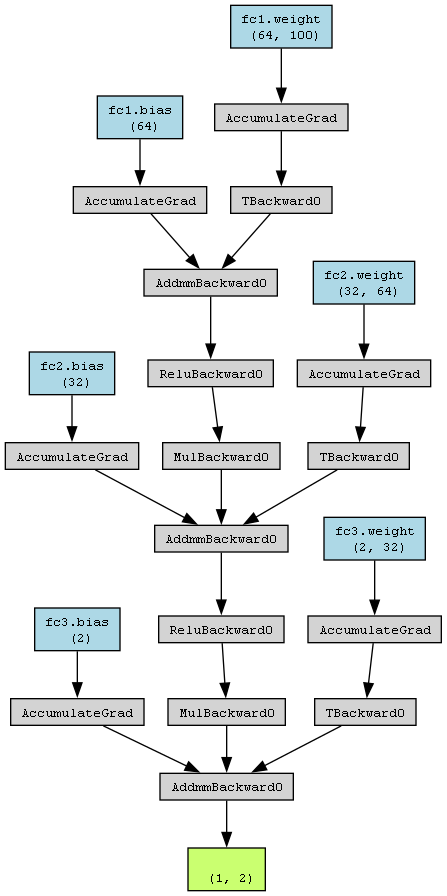
\includegraphics[width=0.4\textwidth]{text_classifier_model.png}
\end{figure}

\subsection{Training process}
True Positives (TP):
\begin{itemize}
  \item Cases that were actually positive (spam) and correctly predicted by the filter to be positive (spam).
  \item Example: An email containing known spam keywords and characteristics is correctly classified as spam by the filter.
\end{itemize}

True Negatives (TN):
\begin{itemize}
  \item Cases that were indeed negative (not spam) and the filter correctly flagged them as negative (not spam).
  \item Example: A regular non-spam email, without any spam-like attributes, is correctly identified as not spam by the filter.
\end{itemize}

False Positives (FP):
\begin{itemize}
  \item Cases that were in fact negative (not spam) but were wrongly flagged by the filter as positive (spam).
  \item Example: A legitimate email from a friend contains certain words or patterns that the spam filter misclassifies as spam.
\end{itemize}

False Negatives (FN):
\begin{itemize}
  \item Cases that were actually positive (spam) but the filter incorrectly flagged them as negative (not spam).
  \item Example: An actual spam email manages to evade detection and is incorrectly classified as a non-spam email.
\end{itemize}

\begin{figure}[H]
    \centering
    \caption{Confusion Matrix}
    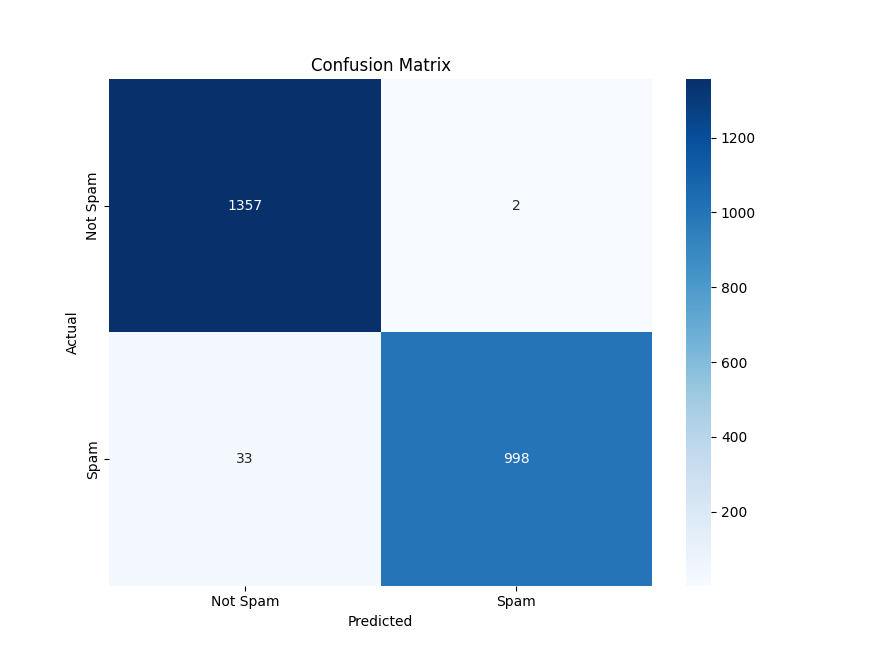
\includegraphics[width=1.1\columnwidth]{confusion_matrix.png}
\end{figure}
\indent The confusion matrix provides a visual representation of these variables, making the representation of these values clearer.

\begin{figure}[H]
    \centering
    \caption{Training loss over time}
    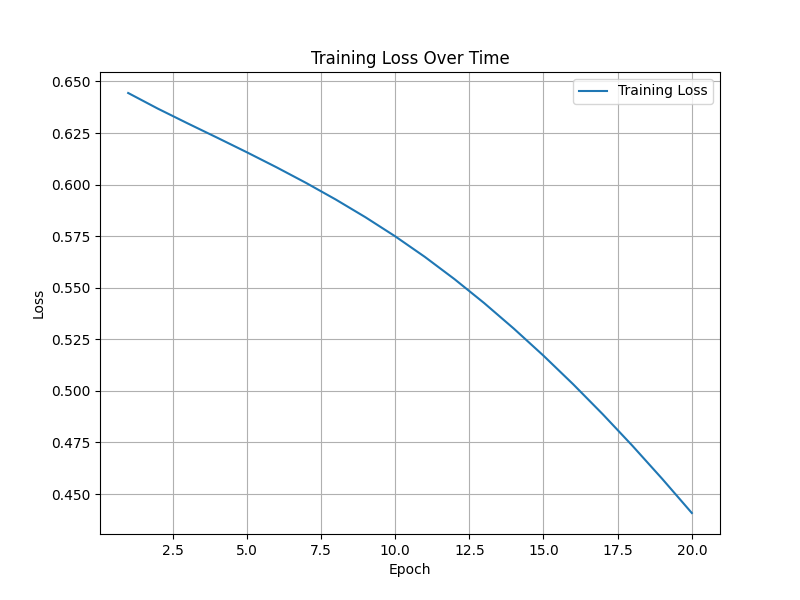
\includegraphics[width=1.1\columnwidth]{training_loss.png}
\end{figure}

\subsection{Evaluation metrics}
\[
\text{Accuracy} = \frac{TP + TN}{TP + TN + FP + FN}
\]
\indent Accuracy measures the overall correctness of the model by calculating the proportion of correctly predicted cases (true positives and true negatives) relative to all cases.

\[
\text{Precision} = \frac{TP}{TP + FP}
\]
\indent Precision is the ratio of correctly predicted positive observations (true positives) to the total number of predicted positives. It focuses on how many of the predicted positive cases were actually positive.

\[
\text{Recall (Sensitivity)} = \frac{TP}{TP + FN}
\]
\indent The recall calculates the ratio of correctly predicted positive observations (true positives) to the total number of true positives. This shows how well the model captures all positive cases.

\[
\text{F1 Score} = 2 \times \frac{\text{Precision} \times \text{Recall}}{\text{Precision} + \text{Recall}}
\]
\indent The F1 score is the harmonic mean of accuracy and recall. It balances accuracy and recall and provides a single metric for evaluating model performance. It is particularly useful when the distribution of classes is uneven.